\documentclass[12pt]{article}

% This first part of the file is called the PREAMBLE. It includes
% customizations and command definitions. The preamble is everything
% between \documentclass and \begin{document}.

\usepackage[margin=1in]{geometry}  % set the margins to 1in on all sides
\usepackage{graphicx}              % to include figures
\usepackage{subfig}
\usepackage{epstopdf}
\usepackage{amsmath}               % great math stuff
\usepackage{amsfonts}              % for blackboard bold, etc
\usepackage{amsthm}                % better theorem environments




\begin{document}

\begin{center}
{\bf \Large Visual Saliency: A Project Proposal}  \\
\vspace{.1in}
{\em Sijie Ling, Shupei Zhang, Mehdi Akbarian Rastaghi}
\end{center}
%\setlength\parindent{0pt}
\section{Introduction}

Visual saliency is the extent of attraction of objects to our visual system. 
The human visual system can focus on the most salient stimuli and pay less attention to the rest. 
For example, a running dog in a still background will attract more of our attention. 
A reason for developing such a feature is that the amount of data we receive through our eyes exceeds our ability to process data. 
Although human brain capabilities evolved through time, it is a big challenge for our brain to process this tremendous amount of data efficiently. 
Hence, visual saliency can help us to identify the most imminent threat, danger, or events needing our attention in general. 
Technically, it reduces the load on our visual system. 

The study of visual saliency can help us to have a deeper understanding of the human visual system. 
Researching in this area can lead to many applications, such as image/video segmentation, image/video compression, foreground annotation, perceptual quality assessment, etc \cite{congReviewVisualSaliency2019}.  
To shed more light, let's start with a case. 

Most of the current video coding methods are using block-based compression. 
As an example, spatial and temporal redundancy is reduced through intra-frame coding and inter-frame coding, respectively\cite{sullivanOverviewHighEfficiency2012}. 
While these methods play a vital role in the comparison area, video encoders can further increase the compression ratio by incorporating visual saliency models. 
This can be achieved by decreasing the quality of regions of low interest, like the background. 
Because it is hard for us to notice the changes in those regions, the perceptual visual quality will likely remain the same.

Another advancement of visual saliency is in the game industries. 
Visual saliency study might help game developers in optimizing the performance of their games. 
Due to the difference in attraction of different regions, not all areas need to be rendered in the highest quality, which leads to a better graphics performance. 
Therefore, considering all contribute of visual saliency techniques motivates us to do some research in this area. 

In this project, we will explore how to use attention mechanisms in computer vision, like \cite{zhangSelfAttentionGenerativeAdversarial2019a},
to help capture global dependencies, and thus improve the saliency prediction performance. 
The model will be an end-to-end model, where the input is an color image and the output is a saliency map.
The saliency map will be the same size as the input image, with scores from 0 to 1 assigned to 
every pixel, indicating the extent of attration of that pixel in the input image.
Higher values corresponds to high visual saliency level.
One example of the original image and its corresponding saliency map is shown in Figure \ref{img:data_example}.



\section{Related Work}

Visual saliency detection methods can be categorized into two two classes: bottom-up models and top-down models \cite{congReviewVisualSaliency2019}.
Before deep learning was widely applied in this field, most of the early methods are bottom-up models.
Those early methods usually involve biological and psychological research about visual attention mechanism. And those two approaches match the common beliefs about biological process of human vision.
In general, those models try to establish links between visual saliency and low-level image features, such as color, contrast, brightness etc. The Itti. model\cite{ittiModelSaliencybasedVisual1998}
is one of the earliest model of this kind, which predicts visual saliency from linear combination of features calculated from color, intensity and orientation.
Some other techniques are also used to achieve better results, such as frequency domain analysis, sparse representation, cellular automata etc. \cite{congReviewVisualSaliency2019}

Top-down models, in the other hand, try to find what factors have the most impact on visual saliency. Those models use visual saliency datasets, which contain images and their saliency annotations
, and analyze them in a data-driven fashion.
In recent years, deep learning is introduced into this area and has boosted the performance of saliency prediction a lot.
Vig et al. \cite{vigLargeScaleOptimizationHierarchical2014} proposed the first neural network for saliency prediction, combining convolutional neural network (CNN) and support vector machine (SVM). Later, researchers start to use transfer learning for saliency 
detection tasks. Very deep convolutional networks (VGG) is used in multiple models \cite{kruthiventiDeepFixFullyConvolutional2015, kummererDeepGazeIIReading2016, corniaPredictingHumanEye2018}, and some of them incorporate gaussian prior for performance improvement.
Generative adversarial networks also achieve good results in saliency prediction \cite{panSalGANVisualSaliency2018, cheHowGazeInfluenced2020}.

Transformers were first applied in natural language processing (NLP) for their ability to model long range and multi-level information \cite{bahdanauNeuralMachineTranslation2016a, vaswaniAttentionAllYou2017a}.
They are later introduced for computer vision tasks and show strong potential in modeling non-local dependencies in images \cite{zhangSelfAttentionGenerativeAdversarial2019a}.
But this technique has not been applied in visual saliency tasks so far.

Our trial of applying attention mechanism to CNNs to improve the performence also has supporting evidence from the aspect of cognitive psychology. There are two contradictory models that try to explain human attention mechanism \cite{gazzaniga2006cognitive}. 
In the “Early Selection Model”, complete analysis is not necessary for an unimportant stimulus before it is excluded from our focus area, while in the “Late Selection Model”, all the stimuli are equally processed until they reach at least the semantic level. 
Both models have evidence and the key to solving the divergence is to find the threshold between them. From this view, since CNN usually have small receptive fields in the first few layers, the information is highly abstract for high level analysis, so traditional models can be regarded as similar to the late selection. 
The computer vision attention mechanism focuses more on global information, and we guess that its low level of preprocessing can ease the burden of CNN and guide it to a better result.

\section{Data}
\subsection{Data Sets}

The data sets that are commonly used for image saliency detection tasks are MIT1003 \cite{judd2012benchmark}, CAT2000 \cite{borji2015cat2000} and SALICON \cite{jiang2015salicon}.
In all these three data sets, the original data are normal pictures with a dimension of about 1000. Grey margins are attached to some of the pictures to make them the same size. 
The labels, or the training targets are heatmaps that highlight some regions that are of interest from experiment data of human.
Generally, those datasets are created using eye-tracking devices. The trajectories of eye movement while
observing the test images/videos are recorded by such devices, and fixation maps can be created
by placing the trajectory as white pixels on a black background. Saliency maps are generated by
applying a gaussian filter to the fixation maps and then normailize the results to range $[0, 1]$.
\begin{figure}
    \centering
    \subfloat[][Original]{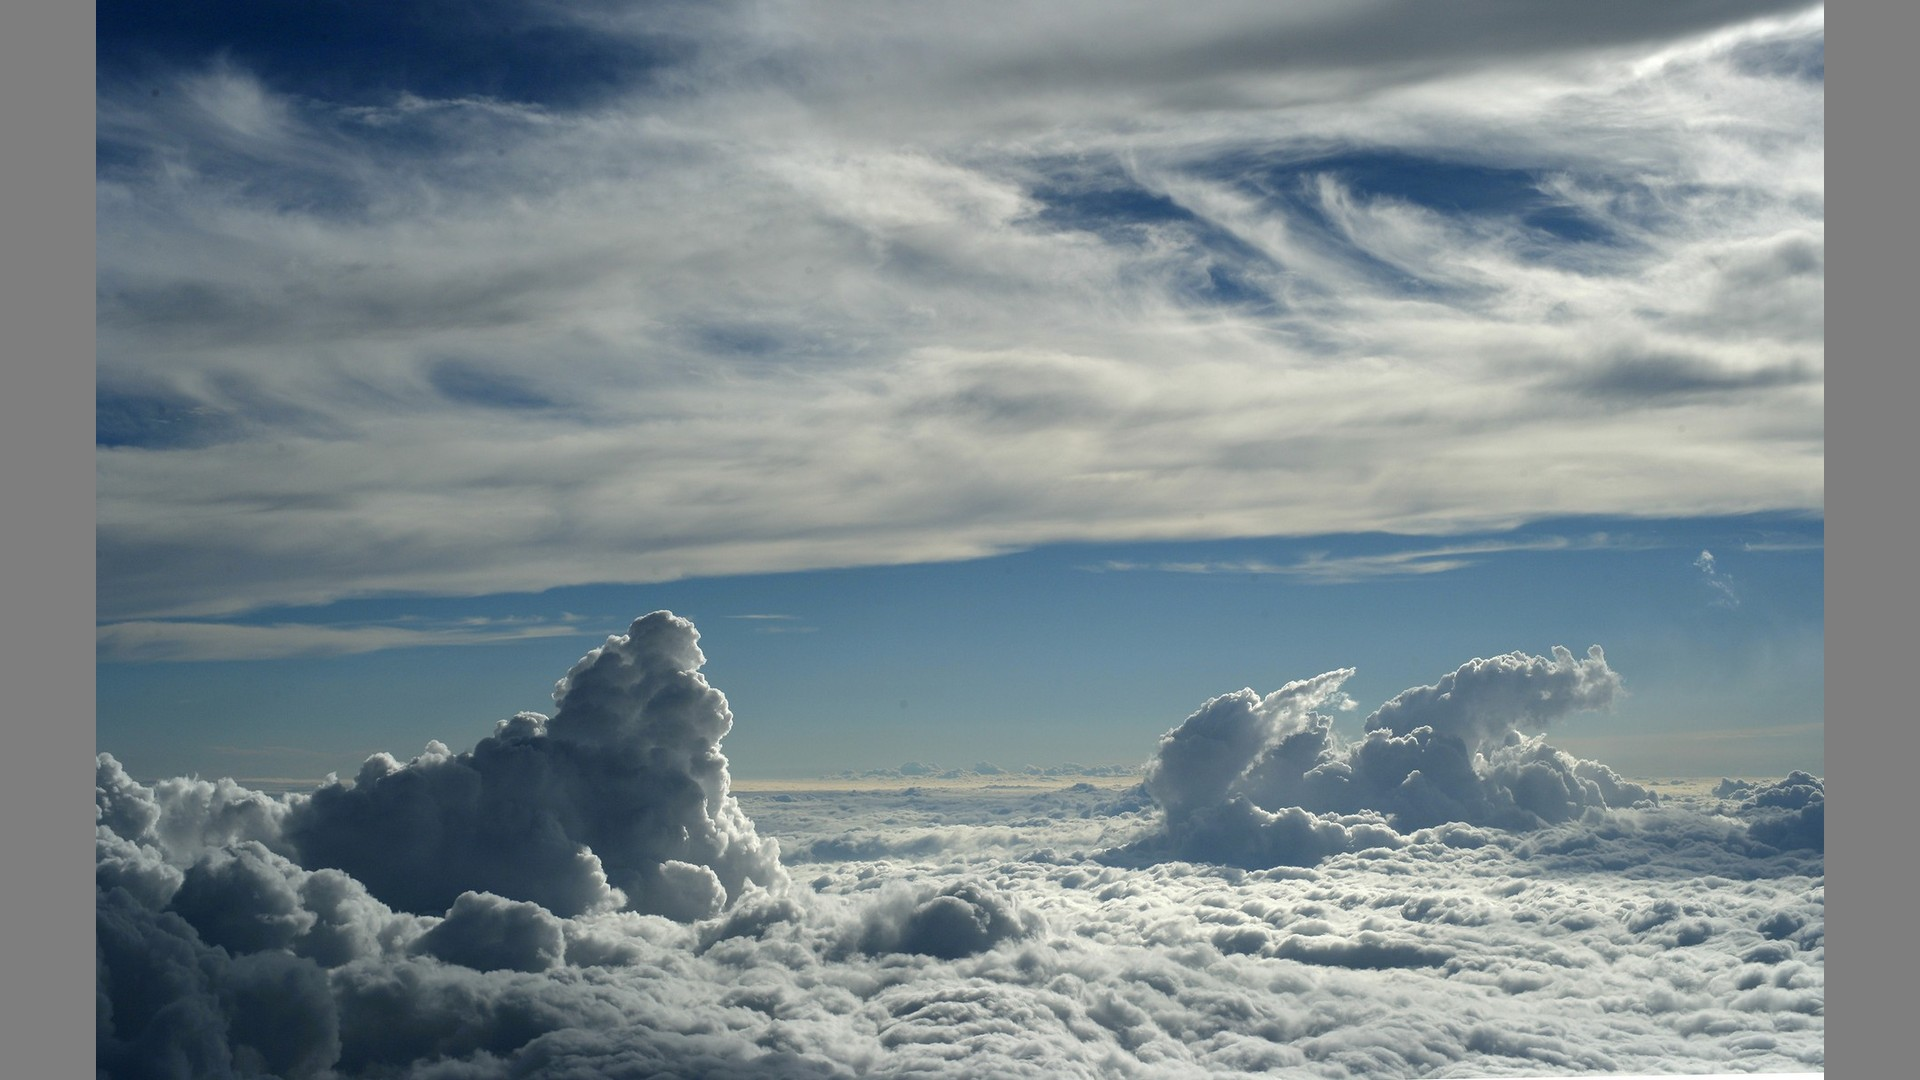
\includegraphics[width=3in]{imgs/Original.jpg}}
    \hspace{5mm}
    \subfloat[][Saliency map]{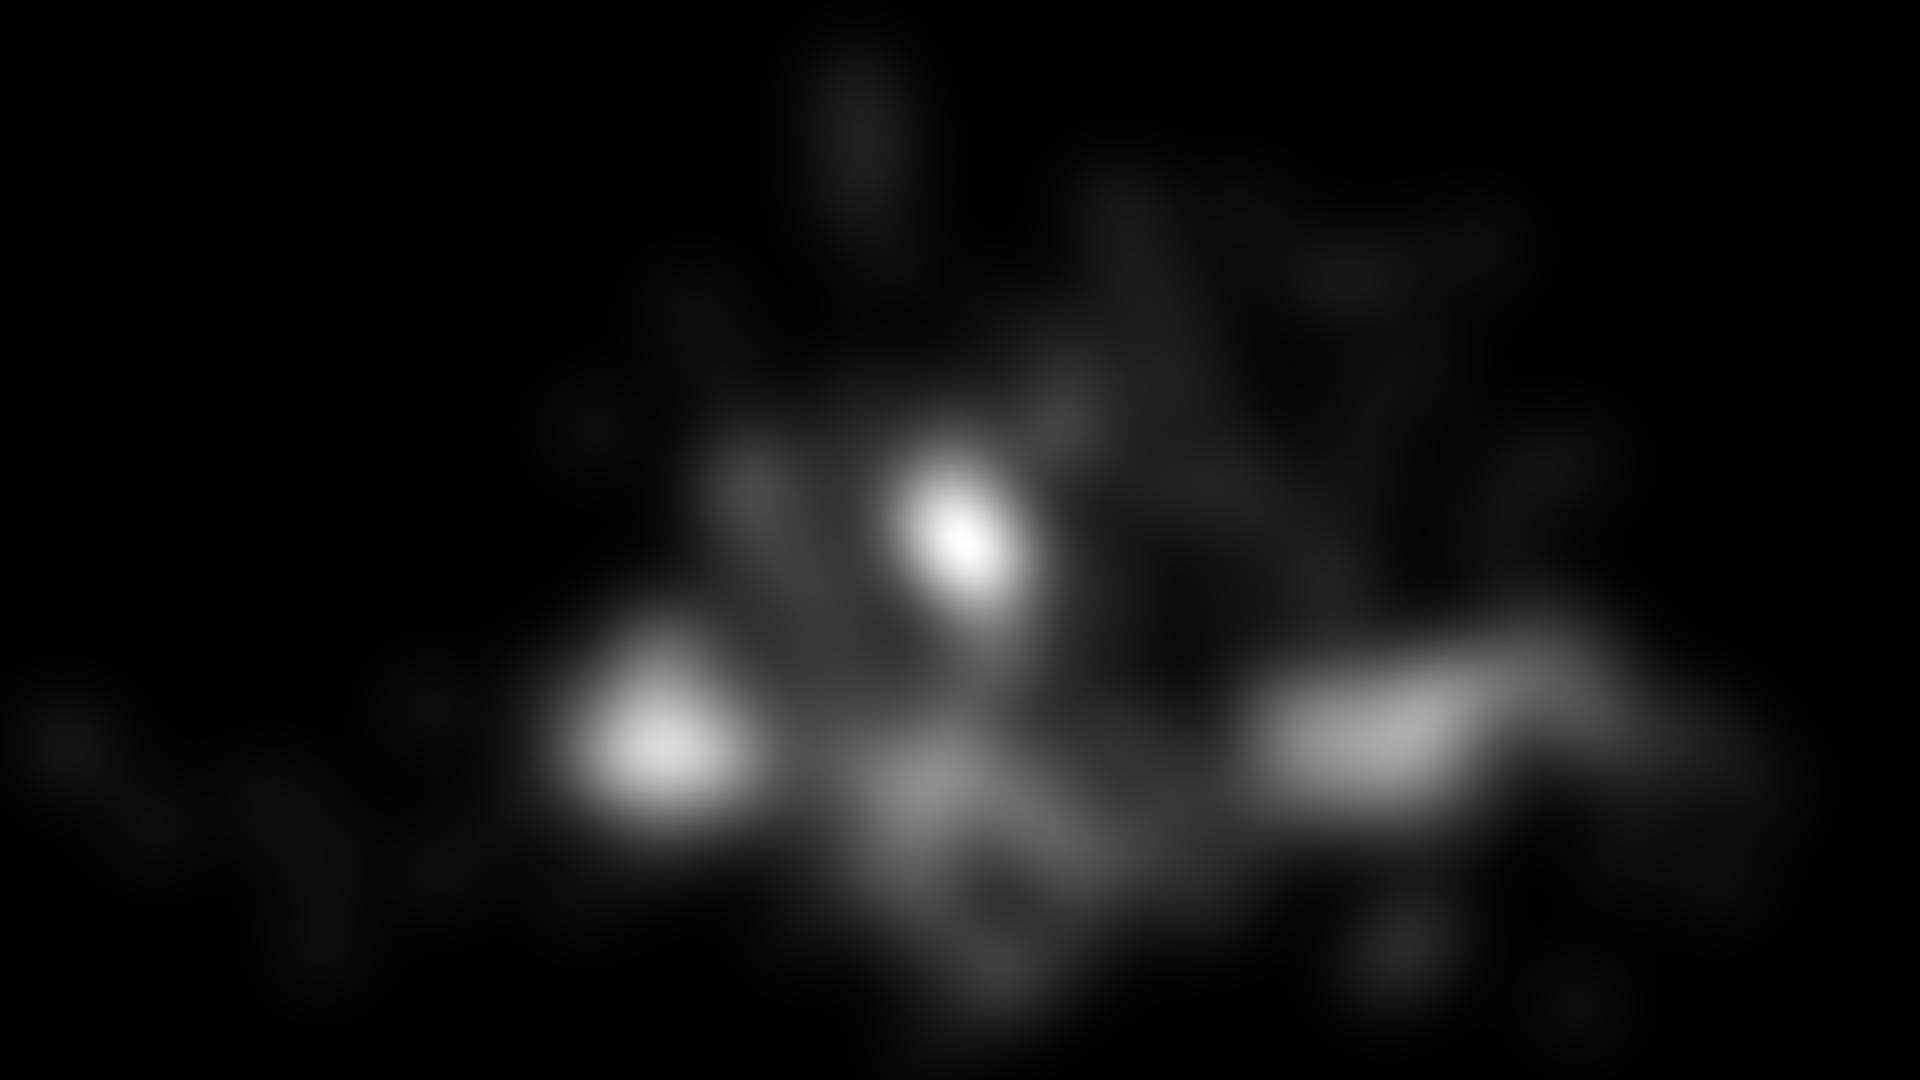
\includegraphics[width=3in]{imgs/FixationMap.jpg}}
    \caption{Data example}
    \label{img:data_example}
\end{figure}

The variety of the public parts of these three data sets are also different. MIT1003 is mainly composed of sceneries and portraits, while the 10,000 figures of SALICON are divided to 100 categories by the objects in them. CAT2000 is more challengeable because it has pictures even in different style, like sketch or inversed photo. 
It must be mentioned that the labels of SALICON is obtained by mouse clicking on rather than eye tracking. Therefore, the distributions of heatmaps are correlated but have minor differences from those of the other two data sets.

\subsection{Interpretability}

Since this task is a regression task rather than a classification task, the output heatmaps can partly explain themselves. 
However, since we are doing analysis on existing CNN framework and use “attention” mechanism as a part of our framework, we should carefully analyze the contribution of these two components. 
Besides comparing the result with their separate performance, we would also disable or disturb the attention mechanism on the trained model to infer their separate roles and cooperation in this task.

Since the heatmaps usually have smoothed margin, when we are doing cross validation or creating random maps to verify our results, it is not appropriate to simple assign random values to create a fake heatmap. 
The random maps that will be used for comparison should also resemble the distribution of heatmaps in the data set.

\section{Analysis}
\subsection{Algorithm}

We can use VGG, ResNet, MobileNet etc. as the backbone of our model, since existing models seem to be fairly simple. Before the picture is directly sent into the framework, an attention framework will firstly assign weights to different parts of the picture.
Another alternative is we can incorporate attention mechanism \cite{zhangSelfAttentionGenerativeAdversarial2019a} into saliency detection model.

Some datasets might not have heatmap groundtruth available, and different dataset might use different gaussian standard variance to create the heatmap.
So we might need to generate heatmaps using a set of uniformed parameters from fixation data.
The training process will be similar to that in most computer vision tasks. Input data is feeded to the model,
and the output is compared with groundtruth to compute loss. Loss is then backpropagated to update model parameters.
Since real test set of these data sets are not public, we will divide the original data set into the train set and the test set. We can use cross validation to choose suitable hyper-parameters on the train set.


\subsection{Performance Measurement}

There are several metrics that can be used to measure the performance. According to \cite{riche2013saliency}, these various metrics may reflect different properties of the algorithm.
\begin{itemize}
    \item Normalized scanpath saliency (NSS \cite{petersComponentsBottomupGaze2005})
    \item Correlation coefficient (CC)
    \item Area Under ROC (AUC \cite{richeSaliencyHumanFixations2013})
    \item etc.
\end{itemize}
The effectiveness of the algorithm can be verified by permutation test. We can choose a small subset and for each figure, we will randomly assign the result of another figure and analyze the metrics mentioned above. This can help prevent bias and make sure the result for each picture is unique.

\subsection{Further Verification}

For the trained network, we may first disable the attention mechanism or the CNN framework and compare the several metrics of the output saliency map with previous results. 
This step will show their separate contributions and the properties of output.

The second step is to find out why attention mechanism may help improve the performance. 
Either during training or test process, upon the output of attention mechanism, we can add noise or use the output of another figure to misguide the CNN network. 
This step can show whether the final output depends largely on attention mechanism.

If time permitting, we might also use the Integrated Gradients algorithm (IG) \cite{sundararajan2017axiomatic} to analyze what pixels in the picture contributes to the result. 
It might be interesting if we can find some pixels that are not highlighted but help the machine to focus. 
Besides, since the IG algorithm measures the gradient change from a totally dimmed picture to the original one, we can test the sensitivity of our algorithm.

\section{Work Plan}

Step1: Before the March 4 checkpoint, we are going to write the code of a traditional CNN network and applies attention mechanism to it. 
If time permitting, we can try two or three attention mechanisms that are differently defined to see whether there are some differences. 
This will mainly be done by Shupei and Sijie.

Step2: Before March 25, interpretability analysis will be done on the trained model. Details include cross validation to test both the final output and the influence of attention mechanism. 
This can be done by Shupei and Mehdi.

Step3: Before we submit the final report, we are going to use some other tools to find some other aspects of our model. 
For example, whether there are some pixels that are not focused but help to achieve the result? How will our model respond to partial or dimmed picture? This can be done by Sijie and Mehdi.

\newpage

\bibliographystyle{unsrt}
\bibliography{proposal}


\end{document}
